\documentclass[a4paper]{article}
\setlength{\topmargin}{-1.0in}
\setlength{\oddsidemargin}{-0.2in}
\setlength{\evensidemargin}{0in}
\setlength{\textheight}{10.5in}
\setlength{\textwidth}{6.5in}
\setlength{\parindent}{0pt}
\usepackage{enumitem}
\usepackage{amsmath}
\usepackage{hyperref}
\usepackage{amssymb}
\usepackage{mathtools}
\usepackage{minted}
\usepackage[dvipsnames]{xcolor}
\usepackage{mathpartir}
\newlist{sollist}{itemize}{1}
\setlist[sollist]{label=$\implies$}
\usepackage{algorithm}
\usepackage{algorithmic}
\usepackage{mathtools}
\DeclarePairedDelimiter{\ceil}{\lceil}{\rceil}
\DeclarePairedDelimiter{\floor}{\lfloor}{\rfloor}
\DeclareMathOperator{\Tr}{Tr}
\DeclareMathOperator*{\argmax}{arg\,max}
\DeclareMathOperator*{\argmin}{arg\,min}

\hypersetup{
    colorlinks=true,
    linkcolor=blue,
    filecolor=magenta,      
    urlcolor=cyan,
    pdftitle={Assignment 2},
    pdfpagemode=FullScreen,
    }
\def\endproofmark{$\Box$}
\newcommand{\norm}[1]{\left\lVert#1\right\rVert}
\newenvironment{proof}{\par{\bf Proof}:}{\endproofmark\smallskip}
\begin{document}
\begin{center}
{\large \bf \color{red}  Department of Computer Science} \\
{\large \bf \color{red}  Ashoka University} \\

\vspace{0.1in}

{\large \bf \color{blue} Introduction to Machine Learning: CS-3410-1}

\vspace{0.05in}

    { \bf \color{YellowOrange} Assignment 2}
\end{center}
\medskip

{\textbf{Name: Dhruman Gupta} }

\bigskip
\hrule

\section{Proving the validity of the Kernel}

The feature map $\phi$ is given by:
\begin{equation*}
    \phi_i(x) = \frac{1}{\sqrt{i!}}e^{-\frac{x^2}{2}} x^i
\end{equation*}

For all $i \geq 0$. We need to show that the kernel $K$ defined as:
\begin{equation*}
    K(x, x') = e^{-\frac{(x-x')^2}{2}}
\end{equation*}
is a valid kernel, and infact, $K(x, x') = \langle \phi(x), \phi(x') \rangle$.

\subsection{Showing that $K$ is a valid kernel}

We need to show $K$ is a valid kernel, i.e., the matrix $K_M = [k_{ij}]$ where $k_{ij} = K(x_i, x_j)$ is positive semi-definite.\\

To prove that $K$ is a valid kernel, I will first prove the following claims:\\

\textbf{Claim 1:} If $k_1$ is a valid kernel, then for any function $f$, the function:
\begin{equation*}
    k_2(x, x') = f(x)k_1(x, x')f(x')
\end{equation*}
is also a valid kernel.\\

\textbf{Proof:} Let $k_1$ and $f$ be given. We want to show that the matrix of $k_2$ is positive semi-definite.\\

Let $M$ be the matrix of $k_1$. Then, the matrix of $k_2$ is given by $M' = [m'_{ij}]$, where:
\begin{equation*}
    m'_{ij} = f(x_i)m_{ij}f(x_j)
\end{equation*}

Now, take an abritary vector $\alpha = (\alpha_1, \alpha_2, \ldots, \alpha_n) \in \mathbb{R}^n$, where $n$ is the number of points in the dataset. Then, we have:
\begin{equation*}
    \alpha^T M' \alpha = \sum_{i,j=1}^n \alpha_i \alpha_j m'_{ij} = \sum_{i,j=1}^n \alpha_i \alpha_j f(x_i)m_{ij}f(x_j)
\end{equation*}

Let $\beta = (\beta_1, \beta_2, \ldots, \beta_n) \in \mathbb{R}^n$ be given by $\beta_i = f(x_i) \alpha_i$. Then, we have:
\begin{equation*}
    \alpha^T M' \alpha = \sum_{i,j=1}^n \alpha_i \alpha_j m'_{ij} = \sum_{i,j=1}^n \alpha_i \alpha_j f(x_i)m_{ij}f(x_j) = \beta^T M \beta
\end{equation*}

Now, as $M$ is positive semi-definite, we have $\beta^T M \beta \geq 0$. Thus, for any vector $\alpha \in \mathbb{R}^n$, we have $\alpha^T M' \alpha \geq 0$. Hence, $M'$ is also positive semi-definite. This completes the proof of Claim 1. $\blacksquare$\\


\textbf{Claim 2:} If $k_1$ and $k_2$ are valid kernels, then $k = k_1 * k_2$ is also a valid kernel.\\

\textbf{Proof:} Let $k_1$ and $k_2$ be given. Since these are valid kernels, there exist feature maps $\phi_1$ and $\phi_2$ such that $k_1(x, x') = \langle \phi(x), \phi(x') \rangle$ and $k_2(x, x') = \langle \psi(x), \psi(x') \rangle$.\\

Now, let $\phi$ be the feature map defined as:
\begin{align*}
    \xi(x) &= \phi(x) \otimes \psi(x)
\end{align*}

Which means that:
\begin{align*}
    \xi_{ij}(x) = \phi_i(x) \psi_j(x)
\end{align*}

Now, let's look at $\langle \xi(x), \xi(x') \rangle$:

\begin{align*}
    \langle \xi(x), \xi(x') \rangle &= \sum_{i,j} \xi_{ij}(x) \xi_{ij}(x') \\
    &= \sum_{i,j} \phi_i(x) \psi_j(x) \phi_i(x') \psi_j(x') \\
    &= \sum_{i,j} \phi_i(x) \phi_i(x') \psi_j(x) \psi_j(x') \\
    &= \langle \phi(x), \phi(x') \rangle \langle \psi(x), \psi(x') \rangle \\
    &= k_1(x, x')k_2(x, x')\\
    &= k(x, x')
\end{align*}

This shows that $k$ is a valid kernel, as $\xi$ is indeed the feature map for $k$. $\blacksquare$\\

\textbf{Claim 3:} Let $k_1$ and $k_2$ be valid kernels. Then, $k(x, x') = k_1(x, x') + k_2(x, x')$ is also a valid kernel.\\

\textbf{Proof:} Let $k_1$ and $k_2$ be given. This is elementary: consider the kernel matrices $M_1$ and $M_2$ of $k_1$ and $k_2$ respectively. Then, the kernel matrix of $k$ is given by $M_1 + M_2$. As the sum of two positive semi-definite matrices is positive semi-definite, $k$ is a valid kernel. $\blacksquare$\\

\textbf{Claim 4:} Let $k_1$ be a valid kernel. Then for all $c > 0$, $k(x, x') = ck_1(x, x')$ is also a valid kernel.\\

\textbf{Proof:} Let $k_1$ be given. This is elementary: consider the kernel matrix $M_1$ of $k_1$. Then, the kernel matrix of $k$ is given by $cM_1$. As $M_1$ is positive semi-definite, $cM_1$ is also positive semi-definite. Hence, $k$ is a valid kernel. $\blacksquare$\\

\textbf{Claim 5:} If $k_1$ is a valid kernel, then $k(x, x') = e^{k_1(x, x')}$ is also a valid kernel.\\

\textbf{Proof:} Let's look at the taylor expansion of $k(x, x')$:
\begin{align*}
    k(x, x') = e^{k_1(x, x')} = \sum_{n=0}^{\infty} \frac{k_1(x, x')^n}{n!}
\end{align*}

$k_1$ is a valid kernel, so by Claim 2, $k_1^n$ is also a valid kernel for all $n$. Now, let $c = \frac{1}{n!}$. By Claim 4, $\frac{k_1^n}{n!}$ is a valid kernel.\\

By Claim 3, the sum of valid kernels is a valid kernel. Hence, $k$ is a valid kernel. $\blacksquare$\\

\textbf{Proof for the kernel $K$:} First, let's decompose $K$ as:
\begin{equation*}
    K(x, x') = e^{-\frac{(x-x')^2}{2}} = e^{-\frac{x^2}{2}} e^{-\frac{x'^2}{2}} e^{xx'}
\end{equation*}

Now, we know that the kernel $k(x, x') = \langle x, x' \rangle$ is a valid kernel. Since $x$ is one-dimensional, $\langle x, x' \rangle = xx'$.\\

By Claim 5, $g(x, x') = e^{xx'}$ is a valid kernel. Now, let $f(x) = e^{-\frac{x^2}{2}}$. By Claim 1, $f(x)g(x, x')f(x')$ is a valid kernel.\\

We had that $K(x, x') = e^{-\frac{(x-x')^2}{2}} = e^{-\frac{x^2}{2}} e^{-\frac{x'^2}{2}} e^{xx'}$. I have proven that this is a valid kernel, as:
\begin{align*}
    &f(x)g(x, x')f(x')\\
    &= e^{-\frac{x^2}{2}} e^{-\frac{x'^2}{2}} e^{xx'}\\
    &= e^{-\frac{(x-x')^2}{2}}\\
    &= K(x, x')
\end{align*}

This completes the proof that $K$ is a valid kernel. $\blacksquare$\\

\newpage

\subsection{Proving the feature map}

Let's look at the feature map $\phi$ defined as:
\begin{equation*}
    \phi_i(x) = \frac{1}{\sqrt{i!}}e^{-\frac{x^2}{2}} x^i
\end{equation*}

Taking the dot product of $\phi(x)$ and $\phi(x')$ we get:
\begin{align*}
    \langle \phi(x), \phi(x') \rangle &= \sum_{i=0}^{\infty} \phi_i(x) \phi_i(x') \\
    &= \sum_{i=0}^{\infty} \frac{1}{\sqrt{i!}}e^{-\frac{x^2}{2}} x^i \frac{1}{\sqrt{i!}}e^{-\frac{x'^2}{2}} x'^i \\
    &= \sum_{i=0}^{\infty} \frac{1}{i!}e^{-\frac{x^2}{2}} e^{-\frac{x'^2}{2}} x^i x'^i \\
    &= e^{-\frac{x^2}{2}} e^{-\frac{x'^2}{2}} \sum_{i=0}^{\infty} \frac{1}{i!} x^i x'^i\\
    &= e^{-\frac{x^2 + x'^2}{2}}\sum_{i=0}^{\infty} \frac{1}{i!} (xx')^i
\end{align*}

Now, note that $\sum_{i=0}^{\infty} \frac{1}{i!} (xx')^i = e^{xx'}$. Hence, we have:
\begin{align*}
    \langle \phi(x), \phi(x') \rangle &= e^{-\frac{x^2 + x'^2}{2}} e^{xx'} \\
    &= e^{-\frac{(x-x')^2}{2}} \\
    &= K(x, x')
\end{align*}

This completes the proof that $\phi$ is the feature map for $K$. $\blacksquare$\\

\newpage

\section{More and more SVMs}

\subsection{Perceptron $>$ SVM?}

The question asks us: what is the difference between the Perceptron and the SVM?
\begin{figure}[h]
    \centering
    
\includegraphics[width=0.75\textwidth]{figures/perceptron.jpg}
\end{figure}

The advantages of the hard-margin SVM compared to the Perceptron we discussed are as follows:
\begin{itemize}
    \item The Perceptron is a logistic regression model, but instead of predicting a continuous value, it predicts a binary value. Indeed- it gives a separating hyperplane, that separates the data into two classes.
    \item This hyperplane can be arbritary - close to the data, or far away. It depends on the model, the hyperparameters, and the data.
    \item However, in the case of a hard-margin SVM, the hyperplane is the one that is farthest away from the data. It is the one that maximizes the margin. This solves a clear quadratic programming problem, and is a convex problem - thus, we are guaranteed to find the global minimum.
    \item In the case of the perceptron, we can also converge at local minima, and we are not guaranteed to find the global minimum.
\end{itemize}

The very formulation of the perceptron is different from that of the SVM. The perceptron is a linear model trying to minimise it's loss of predicting the correct class. It does not care about the distance of the hyperplane from the data.\\

Instead of a naive loss function like this, the SVM has a loss function that maximises the margin between the hyperplane and the data. The key benefits we observe are:
\begin{itemize}
    \item The separating hyperplane is the farthest. So new data would like to be classified better, and the model will be better at generalising.
\end{itemize}

However, all of this is of course given the fact that the data is linearly separable. If the data is not linearly separable, the perceptron will converge, but the SVM will not - there will be no hyperplane that can separate the data.


\newpage

\subsection{New formulations}

In class, we discussed the following formulation of the SVM:
\begin{align*}
    \min_{w, b} \norm{w}^2&\\
    \text{subject to } \forall i, \ &y_i(w^T x_i + b) \geq 1
\end{align*}

Now, we are given the following formulation:
\begin{align*}
    \min_{w, b} \norm{w}^2&\\
    \text{subject to } \forall i, \ &y_i(w^T x_i + b) \geq 0\\
    &\min_i | y_i(w^T x_i + b) | = 1
\end{align*}

\textbf{(a) Proving that the optimal solution for A is feasible for B}\\

Let $w, b$ be the optimal solution for A. Then, we have:
\begin{align*}
    \forall i, \ &y_i(w^T x_i + b) \geq 1
\end{align*}

Clearly, the constraint $y_i (w^T x_i + b) \geq 0$ is satisfied. We also know that:
\begin{align*}
    \min_i | y_i(w^T x_i + b) | \geq 1
\end{align*}

Now, assume that $c = \min_i | y_i(w^T x_i + b) | > 1$.\\

Now, define $w' = \frac{w}{c}$ and $b' = \frac{b}{c}$. Then, we have:
\begin{align*}
    \forall i, \ &y_i(w'^T x_i + b')\\
    &= \frac{y_i}{c}(w^T x_i + b)\\
    &\geq \frac{y_i}{c} \cdot 1\\
    &= \frac{y_i}{c}
\end{align*}

This means that $w', b'$ is a feasible solution for A, contradicting the optimality of $w, b$. So, it must be the case that $\min_i | y_i(w^T x_i + b) | = 1$. This completes the proof. $\blacksquare$\\

\textbf{(b) Proving that the optimal solution for B is feasible for A}\\

Let $w, b$ be the optimal solution for B. Then, we have:
\begin{align*}
    &\min_i | y_i(w^T x_i + b) | = 1\\
    \text{and } &\forall i, \ y_i(w^T x_i + b) \geq 0
\end{align*}

Clearly, as $\min_i | y_i(w^T x_i + b) | = 1$, we have:
\begin{align*}
    \forall i, \ &| y_i(w^T x_i + b) | \geq 1
\end{align*}

This implies that $w, b$ is a feasible solution for A. This completes the proof. $\blacksquare$\\

\subsection{Proving that the optimal solution for A is optimal for B and vice versa}

Let $w, b$ be the optimal solution for A. Let $w', b'$ be the optimal solution for B.\\

Now, $w', b'$ is feasible for $A$, as shown in part (b). By optimality of $w, b$, we have:
\begin{align*}
    \norm{w}^2 \leq \norm{w'}^2
\end{align*}

$w'$ was the optimal solution for $B$, so we have:
\begin{align*}
    \norm{w'}^2 \leq \norm{w}^2
\end{align*}

Since $\norm{w}^2 \leq \norm{w'}^2 \leq \norm{w}^2$, we have $\norm{w} = \norm{w'}$. This implies that $w = w'$.\\

This shows that the optimal solution for $A$ is also the optimal solution for $B$, and vice versa. $\blacksquare$\\

\section{Hard and soft margins}

\subsection{Convergence of Hard Margin SVM}

No, the hard-margin SVM does not converge when the data is not linearly separable. This is because it looks for a hyperplane that separates the data, and if the data is not separable, no such hyperplane exists. The optimisation problem does not have a solution, and the algorithm will not converge.

\subsection{Soft Margin SVM}

Let's look at the optimisation problem to define the soft-margin SVM (I have taken this from Andrew Ng's notes):
\begin{align*}
    \min_{w, b} \norm{w}^2 + C \sum_{i=1}^n \xi_i&\\
    \text{subject to } \forall i, \ &y_i(w^T x_i + b) \geq 1 - \xi_i\\
    &\xi_i \geq 0
\end{align*}

Now, the question is what happens when $C \rightarrow \infty$. Now, to minimise this, the optimal solution is to minimise the $\xi_i$'s, because very marginal errors are heavily penalised. So, when $C \rightarrow \infty$, the optimisation problem is equivalent to the hard-margin SVM, i.e $\xi_i = 0\ \forall i$. Note this is the case only when $C$ is actually infinite. But, regardless, as $C \rightarrow \infty$, the optimisation problem becomes more and more like the hard-margin SVM, and the solution converges to the hard-margin SVM.\\

The second case is when $C \rightarrow 0$. Now, to minimise the objective, the $\xi_i$'s can be made arbitrarily large, as they will have almost no penalty. In the extreme case when $C = 0$, the optimisation problem is equivalent to:
\begin{align*}
    \min_{w, b} \norm{w}^2&\\
    \text{subject to } \forall i, \ &y_i(w^T x_i + b) \geq -\infty
\end{align*}

Here, the solution is to simply output $w = 0$. That will still satisfy the constraint, as whatever value $b$ takes, it will be greater than $-\infty$. So, the solution is to output $w = 0$, and $b$ can be anything. This is a degenerate case, and the solution is not useful.


\subsection{Proving that at least one point lie on each supporting hyperplane}

In SVMs, we get the support vectors as the points that lie on the margin. Now, we need to show that at least one point lies on each supporting hyperplane. Consider the two hyperplanes $H_{-}$ and $H_{+}$, which are defined as:
\begin{align*}
    H_{-} &= \{x \mid w^T x + b = -1\}\\
    H_{+} &= \{x \mid w^T x + b = 1\}
\end{align*}

We have from the second formulation of the SVM that:
\begin{align*}
    \min_{i} | y_i(w^T x_i + b) | = 1
\end{align*}

Now, this already implies that at least one point lies on one of the hyperplanes. Now, when referring to the KKT conditions (as explained in Ng's notes), we see that if $\alpha_i > 0$ where $\alpha_i$ is the Lagrange multiplier for the $i$-th point, then it must be the case that $y_i(w^T x_i + b) = 1$. This is because we have:

\begin{align*}
    \alpha_i (1 - y_i(w^T x_i + b)) = 0
\end{align*}

Now, if $\alpha_i > 0$, then it must be the case that $1 - y_i(w^T x_i + b) = 0$, i.e., $y_i(w^T x_i + b) = 1$. Now, we also have that:
\begin{align*}
    \sum_{i=1}^n \alpha_i y_i = 0
\end{align*}

From earlier, we saw that one point is already on the hyperplane, so $\alpha_i > 0$ for at least one $i$. For this sum to be 0, another $\alpha_j$ must be positive, such that $y_j = -y_i$. This means that the point $x_j$ lies on the hyperplane $H_{-}$ if $x_i$ lies on $H_{+}$. This completes the proof. $\blacksquare$\\


\newpage

\section{SVMs - optimisation}

\subsection{$\ell_2$ norm - removing $\xi_i \geq 0$}

Let's first look at the optimisation problem:
\begin{align*}
    \min_{w, b} \frac{1}{2} \norm{w}_2^2 + \frac{C}{2} \sum_{i=1}^n \xi_i ^ 2&\\
    \text{subject to } \forall i, \ &y_i(w^T x_i + b) \geq 1 - \xi_i
\end{align*}

We want to show that removing the $\xi_i \geq 0$ constraint keeps the solution the same. Let $w, b, \xi$ be the solution to the optimisation problem.\\

If $\xi_i \geq 0$ then the constraint is satisfied - so it is equivalent to the original problem. Now, let's look at the case when $\xi_i < 0$. I will show that this is not the optimum solution.\\

Consider $\epsilon_i = \max{0, \xi_i}$. We know that $\xi_i$ are feasible and optimal, so:
\begin{align*}
    y_i(w^T x_i + b) \geq 1 - \xi_i \geq 1 - \epsilon_i
\end{align*}

So with our new $\epsilon_i$, the constraint is satisfied. Now, let's look at the objective:
\begin{align*}
    \frac{1}{2} \norm{w}_2^2 + \frac{C}{2} \sum_{i=1}^n \xi_i ^ 2 \geq \frac{1}{2} \norm{w}_2^2 + \frac{C}{2} \sum_{i=1}^n \epsilon_i ^ 2
\end{align*}

This is because if any $\xi_i < 0$, then $\epsilon_i = 0$, and the term vanishes. Thus, by replacing those $\xi_i$ with $0$, we infact have a better solution. Thus, this cannot be the optimal solution. $\blacksquare$\\

\subsection{Lagrangian Formulation}

The lagrangian is given by:
\begin{align*}
    L(w, b, \xi, \alpha, \beta) = \frac{1}{2} \norm{w}_2^2 + \frac{C}{2} \sum_{i=1}^n \xi_i ^ 2 + \sum_{i=1}^n \alpha_i \left[ y_i (x^T w + b) - 1 + \xi_i \right] - \sum_{i=1}^n \beta_i \xi_i
\end{align*}

The multipliers are $\alpha_i \geq 0$ and $\beta_i \geq 0$. 

\subsection{Solving the Lagrangian}

Setting $\nabla_w L = 0$, we get:
\begin{align*}
    \nabla_w L = w - \sum_{i=1}^n \alpha_i y_i x_i = 0 \Rightarrow w = \sum_{i=1}^n \alpha_i y_i x_i
\end{align*}

Setting $\nabla_b L = 0$, we get:
\begin{align*}
    \nabla_b L = \sum_{i=1}^n \alpha_i y_i = 0
\end{align*}

Setting $\nabla_{\xi_i} L = 0$, we get:
\begin{align*}
    \nabla_{\xi_i} L = C\xi_i + \alpha_i - \beta_i = 0 \Rightarrow \xi_i = \frac{\beta_i - \alpha_i}{C}
\end{align*}

\newpage

\section{Kernel Ridge Regression}

\subsection{Closed form solution}

Let $X \in \mathbb{R}^{n \times d}$ be the data matrix, and $y \in \mathbb{R}^n$ be the labels. Our regression loss is given by:
\begin{align*}
    j(\theta) = \sum_{i=1}^n (y_i - \theta^T x_i)^2 + \frac{\lambda}{2} \norm{\theta}_2^2
\end{align*}

Taking the gradient of the loss, we get:
\begin{align*}
    \nabla j(\theta) &= -2\sum_{i=1}^n (y_i - \theta^T x_i)x_i + \lambda \theta\\
    &= -2X^T (y - X\theta) + \lambda \theta
\end{align*}

Setting the gradient to 0, we get:
\begin{align*}
    -2X^T (y - X\theta) + \lambda \theta = 0\\
    \lambda \theta = 2X^T (y - X\theta)\\
    \lambda \theta = 2X^T y - 2X^T X\theta\\
    (\lambda I + 2X^T X)\theta = 2X^T y\\
    \theta = (2X^T X + \lambda I)^{-1} 2X^T y
\end{align*}

This makes an assumption that $(2X^T X + \lambda I)$ is invertible.

\subsection{Kernels!}

We now have kernels, so we can use them to solve the problem. Let's look at the kernel ridge regression problem:
\begin{align*}
    J(\theta, \phi) = \sum_{i=1}^n (y_i - \theta^T \phi(x_i))^2 + \frac{\lambda}{2} \norm{\theta}_2^2
\end{align*}

Define $\psi = \left[ \phi(x_1), \phi(x_2), \ldots, \phi(x_n) \right]$. This means $\psi$ is a $D \times n$ matrix, where $D$ is the dimensionality of the feature space $\phi(x_i)$. The term $\theta^T \phi(x_i)$ is equivalent to the $i$-th entry of $\psi^T \theta$. So the loss can be written as:
\begin{align*}
    J(\theta, \psi) = \norm{y - \psi^T \theta}_2^2 + \frac{\lambda}{2} \norm{\theta}_2^2
\end{align*}

Now, we can use the closed form solution for ridge regression to get:
\begin{align*}
    \theta &= [( \lambda I + 2\psi\psi^T)^{-1} (2\psi) ] y \\
    &= (2\psi) (\lambda I + 2\psi^T\psi)^{-1} y \\
    &= 2\psi (\lambda I + 2K)^{-1} y
\end{align*}

This shows that $\theta$ is a linear combination of the mapped data points $\phi(x_i)$, as $\theta = \psi \alpha_{coeffs}$. Specifically:
\begin{align*}
    \theta = \sum_{i=1}^n (\alpha_{coeffs})_i \phi(x_i)
\end{align*}
Comparing $\theta = \psi \alpha_{coeffs}$ with $\theta = 2\psi (\lambda I + 2K)^{-1} y$:
\begin{align*}
    \alpha_{coeffs} = 2(\lambda I + 2K)^{-1} y = 2(\lambda I + 2\psi^T\psi)^{-1} y
\end{align*}
Now, when predicting for a new input $x_{test}$, we compute $y_{pred}(x_{test}) = \phi(x_{test})^T \theta$:
\begin{align*}
    y_{pred}(x_{test}) &= \phi(x_{test})^T \psi \alpha_{coeffs}
\end{align*}
Let $k(x_{test})^T$ be the $1 \times n$ row vector where its $j$-th element is $K(x_{test}, x_j) = \phi(x_{test})^T \phi(x_j)$. Thus, $k(x_{test})^T = \phi(x_{test})^T \psi$.
The prediction becomes:
\begin{align*}
    y_{pred}(x_{test}) &= k(x_{test})^T \alpha_{coeffs} \\
    &= k(x_{test})^T \left( 2(\lambda I + 2K)^{-1} y \right) \\
    &= 2 k(x_{test})^T (\lambda I + 2K)^{-1} y
\end{align*}
This prediction uses the kernel function $K(x, x')$ for the new input $x_{test}$ against all training samples $x_i$ (contained in $k(x_{test})^T$), the matrix $K = \psi^T\psi$ of the training data, the training labels $y$, and the regularization parameter $\lambda$.\\

So, if $K$ can be computed directly, then we do not need to know the feature map $\phi$.

\newpage

\section{Deep Learning}

\subsection{Decision Bounday}

We want to solve for $\sigma(z) = 0.5$. I will go bottom up in computation. First, let's compute $h_1, h_2$:
\begin{align*}
h_1 &= w_{11}x_1 + w_{12}x_2 + w_{13}\\
&= x_1 - x_2\\
h_2 &= w_{21}x_1 + w_{22}x_2 + w_{23}\\
&= - x_1 - x_2
\end{align*}
Now, let's compute $z$:
\begin{align*}
z &= [v_1, v_2, v_3] \begin{bmatrix}
    f(h_1)\\
    f(h_2)\\
    1
\end{bmatrix}\\
&= \max(0, x_1 - x_2) + \max(0, -x_1 - x_2) - 2
\end{align*}

We want to solve for $\sigma(z) = 0.5$, so $\frac{1}{1 + e^{-z}} = 0.5$. This means that:
\begin{align*}
    1 + e^{-z} &= 2\\
    e^{-z} &= 1\\
    -z &= 0\\
    z &= 0
\end{align*}

Solving for $x_1, x_2$, we get:
\begin{align*}
    2 &= \max(0, x_1 - x_2) + \max(0, -x_1 - x_2)
\end{align*}

So, all solutions that satisfy $\max(0, x_1 - x_2) = \lambda$ and $\max(0, -x_1 - x_2) = 2 - \lambda$ are solutions. Since this is max with 0, both functions are non-negative (so $\lambda \geq 0$ and $2 - \lambda \geq 0$).\\

\textbf{Case 1:} $x_1 - x_2 \leq 0$. Clearly, $\max(0, x_1 - x_2) = 0$. So, we have:
\begin{align*}
    2 &= \max(0, -x_1 - x_2)\\
    &= -x_1 - x_2\\
    x_1 + x_2 &= -2\\
    x_2 &= -2 - x_1
\end{align*}

As $x_1 \leq x_2$, we also have that $x_1 \leq -1$. This means that $x_1 \in (-\infty, -1]$ and $x_2 = -2 - x_1$ is a solution for this case.\\

\textbf{Case 2:} $2 > x_1 - x_2 > 0$. Clearly, $\max(0, x_1 - x_2) = x_1 - x_2 = \lambda$. So, we have:
\begin{align*}
    2 &= \lambda + \max(0, -x_1 - x_2)
\end{align*}
Also, this would mean that $-(x_1 + x_2) > 0$, i.e $x_1 + x_2 < 0$. This means that $x_2 < -x_1$. From our initial constrant, we also get $x_1 > x_2$. So, we have:
\begin{align*}
    -x_2 > x_1 > x_2
\end{align*}

Solving this, we get $2 = x_1 - x_2 -x_1 - x_2 = -2x_2 \Rightarrow x_2 = -1$. Also, $x_1 > x_2 \Rightarrow x_1 > -1$. This means that $x_1 \in (-1, 1)$ and $x_2 = -1$ is the solution for this case.\\

\textbf{Case 3:} \(x_1 - x_2 = 2\) (so \(\lambda = 2\) and the second term is \(0\)).  We must also have \(-x_1 - x_2 \le 0 \iff x_1 \ge -x_2\).\\

$x_2 = x_1 - 2$, and thus $x_1 \ge 1$. 

\textbf{Final Solutions}

Now, putting together all these 3 cases, we get the following solutions:
\[
\mathcal{S} \;=\;
\Bigl\{
(x_1,x_2)\;:\;
\begin{array}{ll}
\text{(i)} & x_1 \le -1,\; x_2 = -2 - x_1,\\[4pt]
\text{(ii)} & -1 < x_1 < 1,\; x_2 = -1,\\[4pt]
\text{(iii)}& x_1 \ge 1,\; x_2 = x_1 - 2
\end{array}
\Bigr\}.
\]
\newpage

A plot of the solutions is given below (plotted using desmos):

\begin{center}
    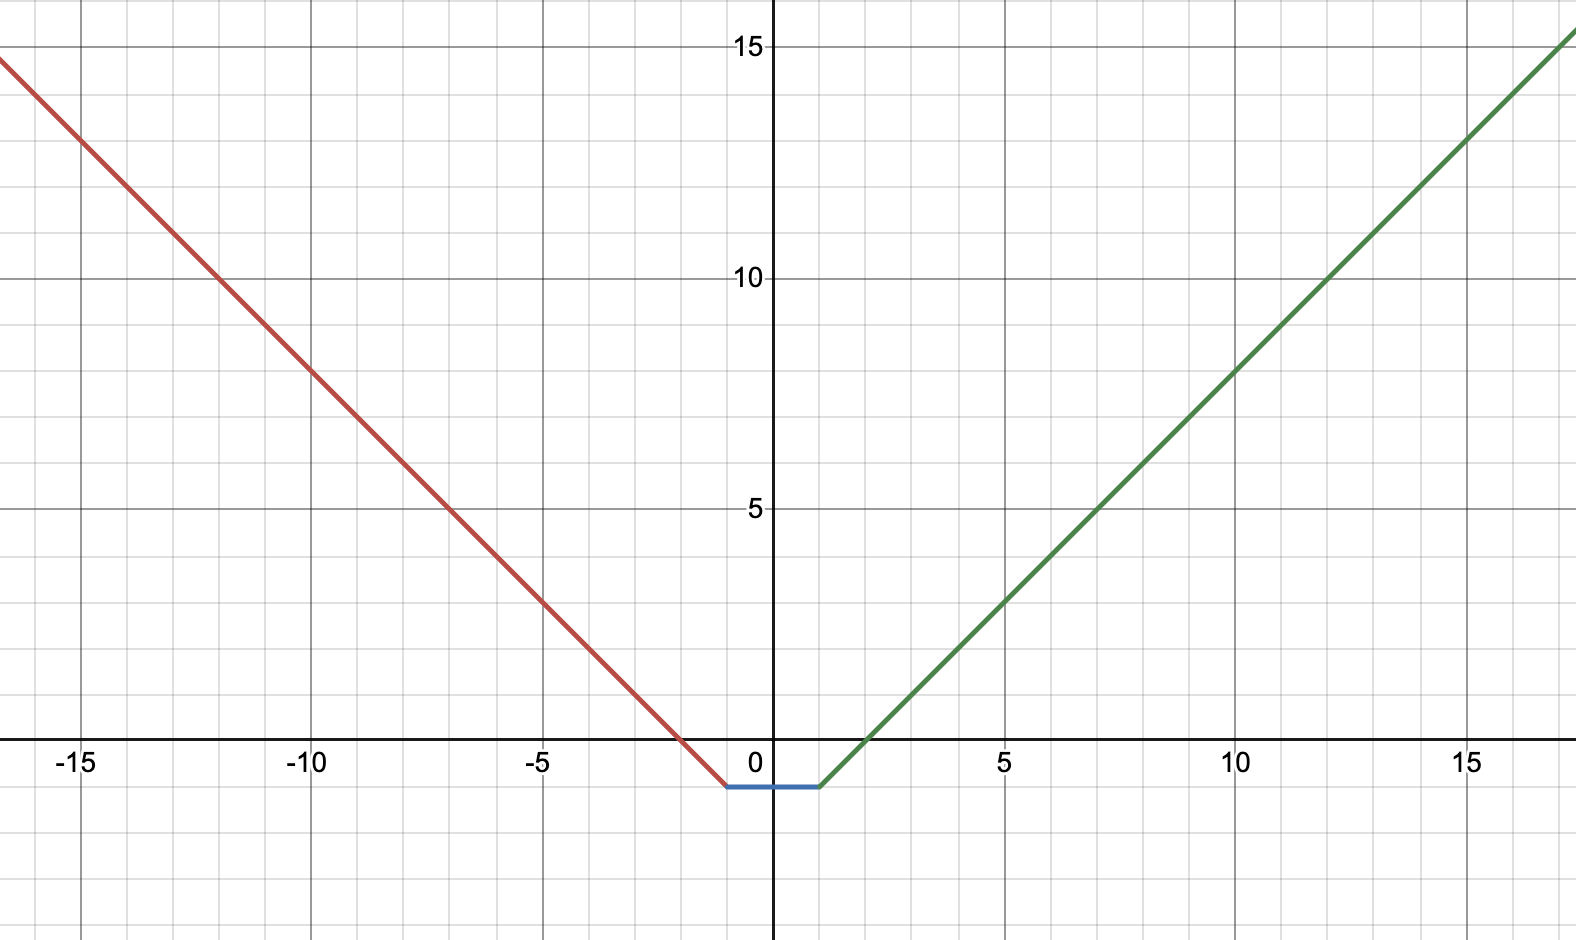
\includegraphics[width=0.75\textwidth]{figures/solutions_boundary.png}
\end{center}

Inside the boundary (i.e above the line), we predict $0$, and outside the boundary (i.e below the line), we predict $1$. Example:

$x_1 = 0, x_2 = 0$. Then, $z = \max(0, 0) + \max(0, 0) - 2 = -2$. Thus, as $z < 0$, we predict $0$.

\subsection{Predicting for $\left[1, 1\right]$}

We have $h_1 = 1 - 1 = 0$ and $h_2 = -1 - 1 = -2$. So, $z = \max(0, 0) + \max(0, -2) - 2 = -2$. Thus, as $z < 0$, we predict $0$.



\end{document}